\documentclass[11pt]{article}
\usepackage[colorlinks,urlcolor=blue]{hyperref}
\usepackage{graphicx}
\usepackage{verbatim}
\setlength{\oddsidemargin}{-0.01in}
\setlength{\topmargin}{-0.4in}
\setlength{\textheight}{9.0in}
\setlength{\textwidth}{6.5 in}
\usepackage{url}

\newenvironment{routine}[2]
{\vspace{.25in}{\noindent\bf\hspace{0pt} #1}{\\ \noindent #2}
\begin{list}{}{
\renewcommand{\makelabel}[1]{{\tt ##1} \hfil}
\itemsep 0pt plus 1pt minus 1pt
\leftmargin  1.2in
\rightmargin 0.0in
\labelwidth  1.1in
\itemindent  0.0in
\listparindent  0.0in
\labelsep    0.05in}
}{\end{list}}


%  \parskip 5pt


\begin{document}

\title{OP2 Developers Guide - Distributed Memory (MPI) Parallelisation}
\author{Mike Giles, Gihan R. Mudalige and Istvan Reguly}

\maketitle

\begin{abstract}
\noindent This document explains OP2's distributed memory parallelisation design and implementation based on MPI.  It is
intended primarily for those who are developing OP2 for distributed memory multi-core CPU and/or GPU clusters and
should be read in conjunction with the OP2 developer manual for single node systems. Those who are only using OP2 should
instead read the Users Manual.
\end{abstract}

\newpage




\tableofcontents

\newpage

\section{Introduction}
The OP2 design uses hierarchical parallelism with two principal levels. At the highest level, OP2 is parallelised across
distributed-memory clusters using MPI message-passing.  This uses essentially the same implementation approach as the
original OPlus. The domain is partitioned among the compute nodes of the cluster, and import/export halos are
constructed for message-passing. Data conflicts when  incrementing indirectly referenced datasets are avoided by
using an ``owner-compute'' model, in which each process performs the computations which are required to update data
owned by that partition. The second level of parallelisation is achieved within a single multi-core CPU or
GPU node. The multi-CPU parallelisation is currently supported by OpenMP threads and in the future will support other
implementations such as Intel's AVX. The GPU support is based on NIVIDIA CUDA and will later support OpenCL. The single
node design and implementation is the subject of the OP2 developer manual. In this document we detail the design of the
distributed memory level based on MPI and describe some of its key implementation aspects. We also detail the
heterogeneous cluster back-end design which facilitates the development and execution of an OP2 application on a cluster
of GPUs and a cluster of multi-threaded CPUs. The Airfoil application supplied with the OP2 release is used as an
example to illustrate the design and implementation.



\section{MPI parallelisation strategy}
% parallel start-up
\subsection{Parallel Startup}\label{subsec/startup}
An OP2 application executed under MPI on a cluster of nodes, where a node may
consist of a single CPU core, a multi-core CPU (or an SMP node) or a GPU node,
will have multiple copies of the same application program executed as separate
MPI processes. The starting point of a distributed memory parallel application
is the design of how the sets, mappings and data on sets that defines an
unstructured mesh application is read in by OP2. The current implementation
achieve this input (and output) via two approaches:
\begin{enumerate}
\item Allow the application developer handles the file I/O where a minor
extension to the OP2 API will makes it possible to define \texttt{op\_set}s,
\texttt{op\_dat}s and \texttt{op\_map}s that are distributed across the MPI
universe.
\item Provide HDF5 based parallel I/O routines with which OP2 routines can
read in the sets, data on sets and mappings from a file in a prescribed format.
\end{enumerate}
The rationale for the above is to allow developers to make the trade-off between
ease-of-use and flexibility. Some will want maximum ease-of-use and are prepared
to pay the price of working with HDF5 files with the flat keyword-based
hierarchy. Others will want the flexibility to manage their data storage in
the way they wish, and will accept the additional programming effort this will entail.

In the first case, we assume that the user I/O has resulted in loading the data
on sets and mappings between sets across the distributed memory MPI universe.
The number of set elements (and thus data on sets) or the size of the mapping
tables held by an MPI process is decided by the application programmer. OP2
assumes that only one partition is held by a single MPI process. For example
given $P$ number of processors, $g\_nnodes$ number of nodes and $g\_nedges$
an application programmer can decide to distribute the nodes and edges so that
each process holds $g\_nnodes/P$ nodes and $g\_nedges/P$. Similarly the edge to
node mapping table could be distributed such that process 0 will provide the
first $g\_nedges/P$ entries, process 1 the second $g\_nedges/P$ entries and so
on. When distributing mapping table entries we assume that the MPI process that
holds some set element X will also hold the mapping table entries (belonging
to all the mapping tables) from X. This is effectively a trivial contiguous
block partitioning of the data on sets and mappings, but it is important to note
that this distribution (or partitioning) will not be used for the parallel
computation. OP2 will repartition the data on sets and related mapping tables,
migrate all data on sets and mappings to the correct MPI process and renumber
the mapping tables as needed. The current MPI implementation provides
partitioning routines (as described in Section~\ref{sec/partitioning}) to
support this task.

\noindent After the loading in of data and mapping tables is complete OP2
\texttt{set}, \texttt{map} and \texttt{dat} declarations can be invoked on each
process. This extends the existing API as follows:
\begin{itemize}
\item {\bf op\_decl\_set}: {\tt size} is the number of elements of the set which
will be provided by this MPI process

\item {\bf op\_decl\_map}: {\tt imap} provides the part of the mapping table
which corresponds to its share of the {\tt from} set

\item {\bf op\_decl\_dat}: {\tt dat} provides the data which corresponds to its
share of {\tt set}
\end{itemize}
\noindent An example implementation of the above is given in the Airfoil application (\texttt{airfoil\_plain}) where an
initial  distribution of data on sets and mapping tables are achieved. MPI rank 0 will serially read in to its RAM the
data on sets and mapping tables from \texttt{new\_grid.dat} and then will distribute the part of data and mappings
(using MPI\_Scatter operations) to other processors.\\

\noindent In the second case, OP2 defines an HDF5 file format (described
later in Section~\ref{sec/hdf5}) using which an applications programmer can
create a file containing data and mappings to be used in the OP2 application.
The OP2 API define the following to support reading from such a file:
\begin{itemize}
\item {\bf op\_decl\_set\_hdf5}: similar to {\bf op\_decl\_set} but with {\tt
size} replaced by {\tt file} which defines the HDF5 file from which {\tt size}
is read using keyword {\tt name}

\item {\bf op\_decl\_map\_hdf5}: similar to {\bf op\_decl\_map} but with {\tt
imap} replaced by {\tt file} from which the mapping table is read using keyword
{\tt name}

\item {\bf op\_decl\_dat\_hdf5}: similar to {\bf op\_decl\_dat} but with {\tt
dat} replaced by {\tt file} from which the data is read using keyword {\tt name}
\end{itemize}

\noindent An example use of HDF5 file I/O is also given in the Airfoil application (\texttt{airfoil\_hdf5}).\\

\noindent If the user is responsible for allocating data arrays to pass to \texttt{op\_decl\_map} and
\texttt{op\_decl\_dat} then the MPI back-end will make a copy of this data internally as halo creation needs to realloc
memory (which might invalidate original pointers held at the user application level). At the end of the program the user
is responsible for freeing the allocated memory at the application level, and OP2 will free its internal copy of this
data when \texttt{op\_exit()} is called.\\

\noindent However, if OP2's hdf5 capabilities are used for File I/O then OP2 will be responsible for clean-up of data
arrays at the end of the program.

\newpage


% construction of halo lists
\subsection{Constructing Halo Lists}\label{subsec/halolists}
The OP2 distributed memory parallelisation uses an ``owner-compute'' model
where each MPI process ``owns'' the elements of the partitioned sets. In order
to ensure that the data associated with these sets are ``up-to-date'' it is
necessary to communicate with ``neighbours'' of an MPI process, and perform
redundant computation on some of the elements imported from these neighbours.
The block of data that's exchanged is commonly known as a halo in distributed
memory programming. \\
\indent Consider an example mesh consisting of nodes and cells, with a cell to
node mapping. If a cell is located on a MPI process, then all the nodes making
up the cell must also be present in this (local) process in order to ensure that
when a loop over cells are performed, the owned cell receives all the possible
contributions from its nodes. If at least one of the nodes are not present in
this local process, then it should be imported in from a foreign MPI process.
Conversely, if a node located on an MPI process is part of a cell that resides
in a foreign MPI process, then that cell needs to be imported in to this local
process because it may need to be executed for the local node to receive all the
required contributions.\\
\begin{figure}[!h]\centering\vspace{-10pt}
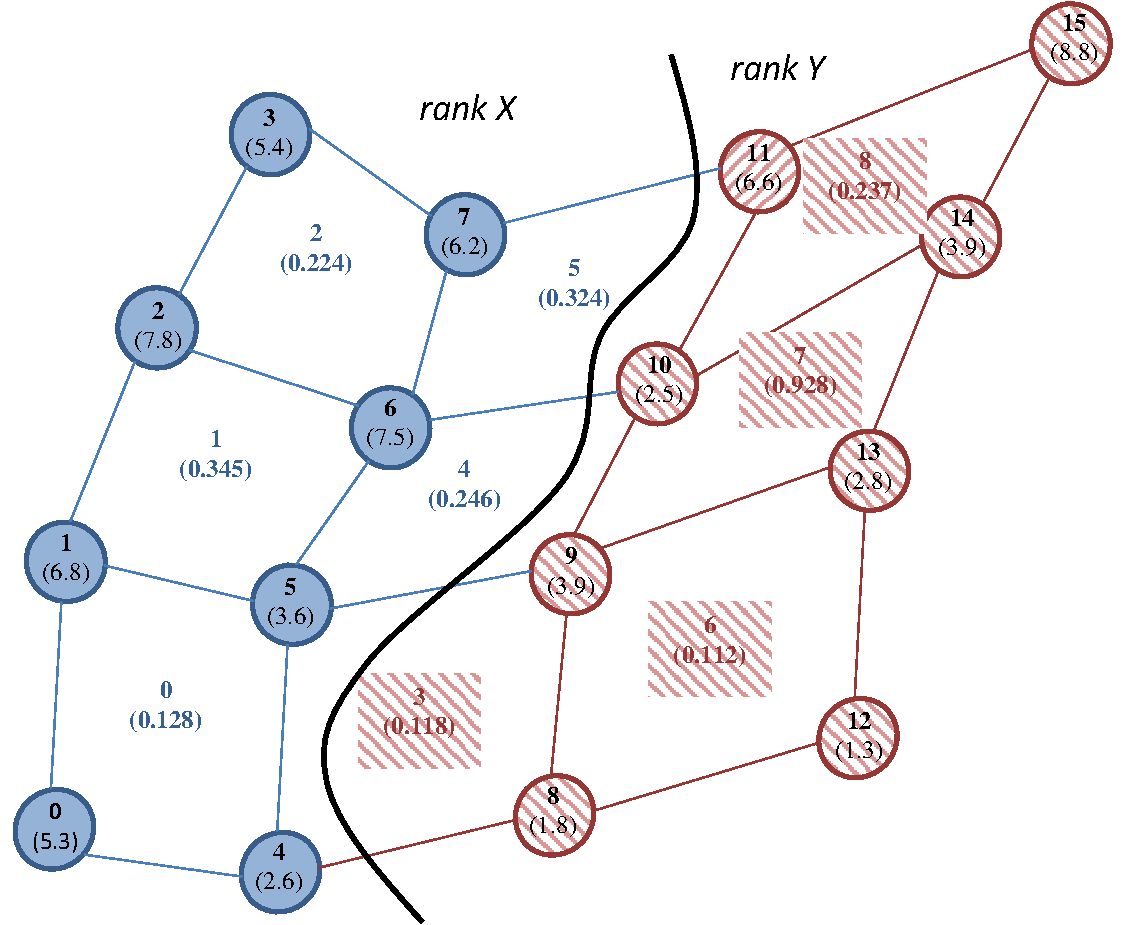
\includegraphics[width=10cm]{mesh-mpidev}\vspace{-0pt}
\caption{Example mesh with cells and nodes}\label{fig/mesh}\vspace{-10pt}
\end{figure}

\noindent In the example mesh illustrated in \figurename{ \ref{fig/mesh}} there
are 16 nodes and 9 cells partitioned across two MPI processes (rank X and rank
Y). Assume that the only mapping available is a cells to node mapping. Rank X
holds nodes 0, 1, 2, 3, 4, 5, 6 and 7 and cells 0, 1, 2, 4, and 5. Rank Y holds
nodes 8, 9, 10, 11, 12, 13, 14,  and 15 and cells 3, 6, 7 and 8. A loop over the
cells will need data on nodes 9, 10 and 11 to be imported in to rank X from
rank Y. Additionally data on nodes 4 and 5 needs to be imported in to rank Y
from rank X. On the other hand, a loop over nodes with contributions from
surrounding cells will cause cells 4 and 5 to be imported into rank Y and ``kept
up to date'' in order to receive their contributions to nodes 9, 10 and 11.
Given the above scenario, each MPI process needs to construct a list of elements
for each set that needs to be imported from and exported to other
``neighbouring'' MPI processes. Within an OP2 application, creation of these
halos occur immediately after partitioning (see Section~\ref{sec/partitioning}) with a call to
\texttt{op\_halo\_create()}. The remainder of this section illustrates the
design and implementation of this routine and the data structures used.

\noindent In order to determine what elements of a set should be imported or
exported (via MPI Send/Receives) to or from another MPI process, we create the
following classification:
\begin{itemize}
\item \textbf{\textit{core}} : An element of a set is said to be a \textit{core}
element to the MPI process it is located at, if all the elements referenced
through all the mapping tables from this set element is also in the
\textit{core} element set in this MPI process. e.g. In a mesh with nodes and
cells (with a mapping of cells to nodes) a cell held within an MPI process is
\textit{core} to this MPI process if all the nodes referenced by this cell is
also \textit{core} to this MPI process.

\item \textbf{export execute halo (\textit{eeh})}: An element of a set is said
to belong to the ``export execute halo'' if at least one element referenced
through any of the mapping tables from this set element is NOT core to this
(local) MPI process. e.g. In a mesh with nodes and cells (with a mapping of
cells to nodes), if a cell references a node owned by a foreign MPI process then
this cell needs to be exported to the foreign MPI process, because it may need
to be executed on that foreign process to update data on that node. This cell
will fall in to the export execute halo (\textit{eeh}) on the local MPI process
and in turn will form part of the import execute halo (\textit{ieh}) on the
foreign MPI process.

\item \textbf{import execute halo (\textit{ieh})}: If an element of a set is
referenced by an element located at a foreign MPI process then the foreign
element needs to be imported on to this MPI process in order to compute the
correct contributions to the local element. The imported element is said to be
in the import execute halo (\textit{ieh}) of the local MPI process. e.g. In a
mesh with nodes and cells (with a mapping of cells to nodes), if a node on the
local MPI process is referenced by a cell in a foreign MPI process, then the
foreign cell needs to be imported and will be part of the import execute halo
(\textit{ieh}) on the local MPI process.

\item \textbf{import non-execute halo (\textit{inh})}: If an element located at
an MPI process references (via some mapping, including mappings belonging to
the \textit{ieh}) an element that is located on a foreign MPI process, then the
element on the foreign MPI process needs to be imported. The imported element
will fall in to the import non-execute Halo (\textit{inh}) if it is not already
a part of the import execute halo (\textit{ieh}). e.g. In a mesh with nodes and
cells (with a mapping of cells to nodes), if a cell references a node owned by a
foreign MPI process then the referenced node needs to be imported onto this MPI
process. The node will fall into the export non-execute halo \textit{enh} on the
foreign MPI process.

\item \textbf{export non-execute halo (\textit{enh})}: If an element of a set is
referenced by an element located on a foreign MPI process then the data for the
local element needs to be exported on the foreign MPI process (if its not
already in the \textit{eeh}). Any loop over the foreign set element cannot
proceed without getting all the contributions from the elements it refers to.
The exported element is said to be part of the export non-execute halo
(\textit{enh}) on the local MPI process. \textit{enh} is a subset of
\textit{core}. e.g. In a mesh with nodes and cells (with a mapping of cells to
nodes) if a node located on the local MPI process is referenced by a cell in a
foreign MPI process, then the local node needs to be exported to that foreign
process.
\end{itemize}

\noindent The above classification allows us to clearly determine which elements
of a set can be computed over without MPI communications, facilitating
overlapping of computation with communications for higher performance (see
Section~\ref{subsec/exchange}). For the mesh given in \figurename{
\ref{fig/mesh}}, the import/export elements can be separated as in Table~\ref{tab/impexp}.\\


\begin{table}[ht]
\centering\vspace{-10pt}
\caption{Import/Export lists}\small
\begin{tabular}{|c|c|c|c|c|c|} \hline
On X 	& \textit{core}	& \textit{ieh}	& \textit{eeh} 	& \textit{inh}	&
\textit{enh} 	\\\hline
Nodes	& 0, 1, 2, 3, 4, 5, 6, 7	& -	& -	& 8, 9, 10, 11	& 4, 5,
6, 7	\\\hline
Cells	& 0, 1, 2			& 3	& 4, 5	&	&\\\hline\hline
On Y 	& \textit{core}	& \textit{ieh}	& \textit{eeh}	& \textit{inh} & enh
\\\hline
Nodes	& 8, 9, 10, 11, 12, 13, 14, 15	& -	& -	& 4, 5, 6, 7	& 8, 9,
10, 11 	\\\hline
Cells	& 6, 7, 8	& 4, 5	& 3	& -		& - \\\hline
\end{tabular}\label{tab/impexp}\vspace{-0pt}
\end{table}\normalsize

\noindent The \texttt{op\_halo\_create()} routine (defined in \texttt{op\_mpi\_core.c}) goes through all the mapping
tables and creates lists that hold the indices of the set elements that fall in to each of the above categories. An
export or an import list for an \texttt{op\_set} has the following structure (defined in \texttt{op\_mpi\_core.h} and
\texttt{op\_mpi\_core.c}):\vspace{-0pt}
\begin{verbatim}
typedef struct {
  op_set set;     //set related to this list
  int size;       //number of elements in this list
  int *ranks;     //MPI ranks to be exported to or imported from
  int ranks_size; //number of MPI neighbors to be exported to or imported from
  int *disps;     //displacements for the starting point of each rank's
                  //element list
  int    *sizes;  //number of elements exported to or imported from each ranks
  int    *list;   //the list of all elements
} halo_list_core;

typedef halo_list_core * halo_list;

halo_list *OP_export_exec_list;//eeh list
halo_list *OP_import_exec_list;//ieh list

halo_list *OP_import_nonexec_list;//inh list
halo_list *OP_export_nonexec_list;//enh list
\end{verbatim}
% \newpage
\noindent The above four arrays are indexed using \texttt{set->index} and is of
size \texttt{OP\_set\_index}. Import and export list creation in
\texttt{op\_halo\_create()} is accomplished in the following steps, by each MPI
process:
\begin{enumerate}
\item \textbf{Create export lists for execute set elements}\\
Each MPI process goes through each element of each set. If a set element
references (via any of the mapping table from this set) any element that is not
\textit{core} to the local MPI process then we add the \underline{referencing}
element to the \textit{eeh} list. When creating the \textit{eeh} list on a given
(local) MPI process, we also keep track of the foreign MPI processes that it
will be exported to. The list of elements to be sent to each foreign MPI process
will be sorted according to its local index.

\item \textbf{Create import lists for execute set elements and related mapping
table entries}\\
Each MPI process exchanges the \textit{eeh} list with the relevant neighbour
processes and use the imported lists to construct the \textit{ieh}.

\item \textbf{Exchange mapping table entries using the import/export lists}\\
The \textit{eeh} and \textit{ieh} on each MPI process can now be used to
exchange the bits of the mapping tables that are related to the execute halo.
The \textit{eeh} and \textit{ieh} of the ``from set'' of each mapping table is
used to identify which mapping table entries are to be exported and imported.
For each mapping table, the imported mapping table entries will be appended to
the end of the \texttt{op\_map->map} array.

\item \textbf{Create import lists for non-execute set elements }\\
Each MPI process goes through each element of each set, (now using all the
mapping table entries including the additional mapping table entries that were
imported), and adds any other element referenced (but not in \textit{ieh}) to a
\textit{inh} list for each set. The list of elements to be imported from each
foreign MPI process will be sorted according to its local index on the foreign
process.

\item \textbf{Create non-execute set export lists}\\
Each MPI process exchanges the \textit{inh} list with the relevant neighbour
processes and uses the imported lists to construct the \textit{enh}. After this
step, halo lists are complete. Each MPI process has \textit{eeh, enh, ieh} and
\textit{inh} lists.

\item \textbf{Exchange data defined on execute set elements using the set import
or export lists}\\
The data defined on the elements belonging to each halo list is exchanged. The
execute halos are exchanged first. For each \texttt{op\_dat} the imported data
will be appended to the end of the \texttt{op\_dat->data} array.

\item \textbf{Exchange data defined on non-execute set elements using the set
import/export lists}\\
The non-execute halos are exchanged second. For each \texttt{op\_dat} the
imported data will be appended to the end of the \texttt{op\_dat->data} array
after the \textit{ieh} data.

\item \textbf{Renumber Mapping tables}\\
Each MPI process goes through all mapping table entries and renumbers the
referenced set element indices to point to local indices. All required
referenced elements (or a copy of it) should be now available locally on each MPI process.

\item \textbf{Create MPI send buffers}\\
For each \texttt{op\_dat}, create buffer space for \texttt{MPI\_Isend}s.
The following struct holds the required buffers and related data.
\begin{verbatim}
typedef struct {
 int         dat_index;    //index of the op_dat to which
                           //this buffer belongs
 char        *buf_exec;    //buffer holding exec halo
                           //to be exported;
 char        *buf_nonexec; //buffer holding nonexec halo
                           //to be exported;
 MPI_Request *s_req;       //array of MPI_Reqests for sends
 MPI_Request *r_req;       //array of MPI_Reqests for receives
 int         s_num_req;    //number of sends in flight
                           //at a given time for this op_dat
 int         r_num_req;    //number of receives awaiting
                           //at a given time for this op_dat
} op_mpi_buffer_core;

typedef op_mpi_buffer_core *op_mpi_buffer;
op_mpi_buffer *OP_mpi_buffer_list;
\end{verbatim}

\item \textbf{Separate \textit{core} elements}\\
To facilitate overlapping of computation with communication, for each set, the
\textit{core} elements are separated to form a contiguous block of elements. Any
element NOT belonging to the \textit{eeh} is a \textit{core} element. We
rearrange the local set elements and initialise \texttt{set->core\_size} to the
number of core elements. Thus during a loop over a given set, on each MPI
process, element indices \texttt{0} to \texttt{set->core\_size - 1} can be
computed over without halo data and elements from \texttt{set->core\_size}
to \texttt{set->size} + \texttt{OP\_import\_exec[set->index]->size} will need to
be computed over after all the calls to \texttt{wait\_all()} are completed.

\begin{figure}[ht]\centering\vspace{-0pt}\hspace{10pt}
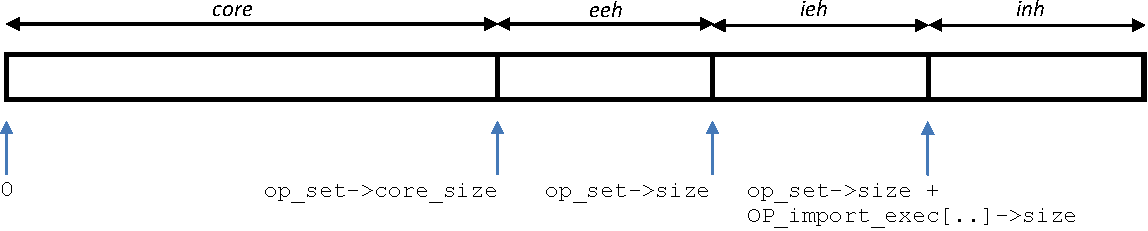
\includegraphics[width=14cm]{elementorder}\vspace{-5pt}
\caption{Element order of an \texttt{op\_set} after halo creation}
\label{fig/elementorganization}\vspace{-0pt}
\end{figure}

\item \textbf{Save the original set element indices}\\
As the set elements are now rearranged, we need to keep track of the original order in which they appeared so that calls
to \texttt{op\_fetch()} as well as final outputs can be accurately handled. The \texttt{part} struct
(see \texttt{op\_mpi\_core.h}) is used to hold the original global indices of each set element.

\item \textbf{Clean up and compute rough estimate of average worst-case halo
size}\\
Temporary arrays are freed and a rough estimate of the average size of
the worst case import halos on each MPI process is computed. This takes in to
account both the \textit{ieh} and \textit{inh} and accounts for the data sizes
held per set element. The calculation does NOT take in to account which halos
are exchanged during the \texttt{op\_par\_loops} later in the application.
\end{enumerate}
\noindent \figurename{ \ref{fig/elementorganization}} illustrates the element
order in which data on a set will be organized after halo creation.


% halo exchange in loops - including overlapping computation and communications
\subsection{Halo Exchanges}\label{subsec/exchange}
% 1. the operation of the par_loop
A call to \texttt{op\_par\_loop} in a OP2 application executed under MPI will result in the loop being executed over the
local elements of the set on each MPI process. Additionally if the loop is an indirect loop, then computation
should be done over the \textit{ieh} as well. Depending on the loop (indirect or direct) and the access type of each
\texttt{op\_arg}, halo exchanges may be needed before computation is performed over any elements that are not
\texttt{core} and in the \texttt{ieh}. After loop computation is performed, depending on the access and argtype of the
\texttt{op\_arg} the halos must be marked as ``dirty'' so that the next iteration of the loop can make the decision to
update the halos as required (defined in \texttt{op\_mpi\_core.c} and \texttt{op\_mpi\_rt\_support.c}). The current
implementation utilise a separate field in the \texttt{op\_dat} struct to holds this information. The value
\texttt{op\_dat->dirtybit} is set to 1 to indicate that the halo of \texttt{op\_dat} has been modified. The rules
governing the loop operation are as follows:
\begin{enumerate}
\item If the \texttt{op\_par\_loop} consists of at least one \texttt{op\_arg}
that is indirectly accessed then the whole loop is classified as an indirect
loop. Else it is a direct loop.

\item Direct loops will only need to loop over the local set size using local
data and no halo exchanges are needed.

\item For indirect loops the following algorithm determines a halo exchange.
\begin{verbatim}
for each indirect op_arg {
  if ((op_arg.access is OP_READ or OP_RW) and (dirty bit is set))
  then do halo exchange for op_arg.dat and clear dirty bit
}
if(all indirect op_arg.access == OP_READ)
   execute/loop over set size
else
   execute/loop over set size + ieh
\end{verbatim}
\item After the loop computation block we set the dirty bit for each
\texttt{op\_arg.dat} with \texttt{op\_arg.access} equal to \texttt{OP\_INC,
OP\_WRITE} or \texttt{OP\_RW}.
\end{enumerate}

\noindent A halo exchange is triggered by a call to \texttt{op\_exchange\_halo(op\_arg* arg)} which is defined in
\texttt{op\_mpi\_rt\_support.c}. Within this call, the above conditions that determines a halo exchange are
checked and if satisfied will pack the relevant halo data to the pre defined send buffers, make a call to MPI
non-blocking operations (\texttt{MPI\_Isend} and \texttt{MPI\_Irecev}) and will return 1 to indicate that a non-blocking
communication is \textit{in-flight}. As detailed in Section~\ref{subsec/halolists}, the \textit{eeh} and the
\textit{enh} of an MPI process provides the indices of the elements that needs to be exported as well as the MPI ranks
that will be exported to. Using these lists an MPI process will pack the data to be set into the send buffers and then
will send them using \texttt{MPI\_Isend} operations. The following is for sending the \textit{eeh}:
\begin{verbatim}
halo_list exp_exec_list = OP_export_exec_list[dat->set->index];

for(int i=0; i<exp_exec_list->ranks_size; i++) {
  for(int j = 0; j < exp_exec_list->sizes[i]; j++)
  {
    set_elem_index = exp_exec_list->list[exp_exec_list->disps[i]+j];
    memcpy(&((op_mpi_buffer)(dat->mpi_buffer))->
    buf_exec[exp_exec_list->disps[i]*dat->size+j*dat->size],
    (void *)&dat->data[dat->size*(set_elem_index)],dat->size);
  }
  MPI_Isend(&((op_mpi_buffer)(dat->mpi_buffer))->
         buf_exec[exp_exec_list->disps[i]*dat->size],
         dat->size*exp_exec_list->sizes[i],
         MPI_CHAR, exp_exec_list->ranks[i],
         dat->index, OP_MPI_WORLD,
         &((op_mpi_buffer)(dat->mpi_buffer))->
         s_req[((op_mpi_buffer)(dat->mpi_buffer))->s_num_req++]);
    }
\end{verbatim}
\noindent The \texttt{MPI\_Isend} operations are immediately followed by
\texttt{MPI\_Irecev} operations, which sets up the non-blocking communications
to directly copy the incoming data in to the relevant \texttt{op\_dat}, using
the \textit{ieh} and \textit{inh} lists.
\begin{verbatim}
halo_list imp_exec_list = OP_import_exec_list[dat->set->index];

int init = dat->set->size*dat->size;
for(int i=0; i < imp_exec_list->ranks_size; i++) {
  MPI_Irecv(&(dat->data[init+imp_exec_list->disps[i]*dat->size]),
         dat->size*imp_exec_list->sizes[i],
         MPI_CHAR, imp_exec_list->ranks[i],
         dat->index, OP_MPI_WORLD,
         &((op_mpi_buffer)(dat->mpi_buffer))->
         r_req[((op_mpi_buffer)(dat->mpi_buffer))->r_num_req++]);
}
\end{verbatim}

\noindent A call to \texttt{op\_wait\_all(op\_arg arg)} routine needs to be performed in order to complete the MPI
communications. The \texttt{op\_par\_loop} is structured so that all the \texttt{op\_exchange\_halo()} calls are done at
the beginning of the loop, followed by computation over the \textit{core} elements of the set and then by calls to
\texttt{op\_wait\_all()}. This will allow for maximum overlapping of computation with communication as none of the
\textit{core} elements reference any halo data. After the calls to the \texttt{op\_wait\_all()} the remaining set
elements could be computed. A reference implementation of the above can be found in \texttt{op\_seq.h}.

% global operations
\subsection{Global Operations}\label{subsec/globalops}

If an \texttt{op\_arg} is of type \texttt{OP\_ARG\_GBL} then a global operation needs to be performed for that argument.
The operation to be performed is one of \texttt{OP\_INC} (global reduction), \texttt{OP\_MAX} (global maximum),
\texttt{OP\_MIN} (global minimum). For an \texttt{op\_arg} of type \texttt{OP\_ARG\_GBL}, the contributions from
executing the \textit{ieh} must not be included. Thus the reference implementation passes in a dummy value in place of
any \texttt{op\_arg} with type \texttt{OP\_ARG\_GBL}. After the loop over the elements are performed on each MPI
process, the global operation should be done across all the MPI processes by a call to \texttt{op\_mpi\_reduce()}. This
routine checks for the type of the data exchanged and the type of the operation to be performed and calls
\texttt{MPI\_Allreduce} with the relevant operation and data type.

% implementing op_fetch and op_put
\subsection{Fetching Data}\label{subsec/putfetch}
The operation of \texttt{op\_fetch\_data ()} within an OP2 application executing over MPI will be to present the current
values of the \texttt{op\_dat}'s data array in the order of the elements that was originally handed to OP2. It should be
noted that the data array presented to the user level application is a \underline{copy} of the current state of the
internal \texttt{op\_dat}. The implementation first makes a copy of the current data values in the \texttt{op\_dat}
requested and will reorder them according to the original global index of the set elements on which this data is defined
on. A similar operation is carried out by \texttt{op\_fetch\_data\_hdf5(op\_dat dat, T* data, int low, int high)} and
\texttt{op\_fetch\_data\_hdf5\_file(op\_dat dat, char const *file\_name)}. See user documentation for more details. \\

\noindent Conversely an \texttt{op\_put\_data()} routine may also be implemented later (as required) so that the user
level application can modify the internal values of an \texttt{op\_dat}. In this case the user submitted data values
will replace the internal \texttt{op\_dat}'s data values. A valid implementation will need to translate the original set
element index to the current set element index.


% performance measurements - including flags to trigger them
\subsection{Performance Measurements}\label{subsec/perf}

For measuring the execution time of code two timer routines are implemented. Firstly, \texttt{op\_timers \_core()} (in
\texttt{op\_lib\_core.c}) measures the elapsed time on a single MPI process while \texttt{op\_timers()}
(in \texttt{op\_mpi\_decl.c}) has an implicit \texttt{MPI\_Barrier()} so that time across the whole MPI universe can be
measured. \noindent The time spent in the \texttt{op\_par\_loop()} calls is measured and accumulated. The setup costs
due to halo creation and partitioning are also measured and the maximum on all the processors is printed to standard out
by rank 0. Additionally information about the amount of MPI communications performed is also collected. For each
\texttt{op\_par\_loop()} we maintain a struct that holds (1) the accumulated time spent in the loop (2) the number of
times the \texttt{op\_par\_loop()} routine is called, (3) the indices of the \texttt{op\_dat}s that requires halo
exchanges during the loop, (4) the total number of times halo exchanges are done for each \texttt{op\_dat} and (5) the
total number of bytes exported for each \texttt{op\_dat}.
\begin{verbatim}
typedef struct
{
  char const  *name;   // name of kernel
  double      time;    //total time spent in this
                       //kernel (compute+comm-overlapping)
  int         count;   //number of times this kernel is called
  int*        op_dat_indices;  //array to hold op_dat index of
                               //each op_dat used in MPI halo
                               //exports for this kernel
  int         num_indices; //number of op_dat indices
  int*        tot_count;   //total number of times this op_dat was
                           //halo exported within this kernel
  int*        tot_bytes;   //total number of bytes halo exported
                           //for this op_dat in this kernel
} op_mpi_kernel;
\end{verbatim}
\noindent Currently, the only way to identify a loop is by its name. Thus we use
a simple hash function on the name string to index into a hash table
(\texttt{op\_mpi\_kernel\_tab[]}) that holds an \texttt{op\_mpi\_kernel} struct
for each loop. Monitoring the halo exchanges require calls to
the \texttt{op\_mpi\_perf\_comm()} (defined in \texttt{op\_mpi\_core.c}) for
each \texttt{op\_arg} that has had a halo exchanged during each call to an
\texttt{op\_par\_loop()}. As this may cause some performance degradation, we
allow the MPI message monitoring to be enabled at compile time using the
\texttt{-DCOMM\_PERF} switch.

\begin{comment}
% output routines
\subsection{Output Routines}\label{subsec/output}
A number of miscellaneous output routines are provided currently, including
routines to output the performance measures, \texttt{op\_timing\_output()} as
well as file writes that directly writes an \texttt{op\_dat} to an ASCI file,
\texttt{gatherprint\_tofile()} or a binary file,
\texttt{gatherprint\_bin\_tofile()}. These routines gathers a
specified \texttt{op\_dat}, (which is distributed across the MPI universe) on to
MPI rank 0 and prints the results to a user specified file. The \texttt{op\_dat}
will be written to file in the same order in which the set elements were handed
to OP2 during the initial input of data and mapping tables. This requires calls
to \texttt{op\_fetch()}.
\end{comment}
% \textbf{op\_get\_size(op\_set set)}

% clean-up routines
\subsection{Garbage Collection}\label{subsec/cleanup}
At the end of the OP2 application a call to \texttt{op\_exit()} will free all halo lists, MPI send buffers and the table
holding performance measures. Also any \texttt{dat}s and \texttt{map}s held internally by OP2 is also freed.

\section{HDF5 File I/O}\label{sec/hdf5}
The current hdf5 file format follows the ASCI file format generated by the naca0012.m Airfoil mesh generator. The
generated hdf5 file structure and contents has can be viewed through the \texttt{h5dump} utility.  The hdf5 I/O routines
that allows to read and write \texttt{op\_set}s, \texttt{op\_map}s, \texttt{op\_dat}s and constants are detailed in the
user documentation.




% \textbf{hdf5 input/output routines} \\
% void op_dump_to_hdf5(char const * file_name)
% void op_get_const_hdf5(char const *name, int dim, char const *type, char*
% const_data,char const *file_name)
% void op_write_const_hdf5(char const *name, int dim, char const *type, char*
% const_data, char const *file_name)


\newpage
\section{Partitioning}\label{sec/partitioning}
Given the unstructured mesh in an OP2 application, distributing the data on sets and mapping tables across the MPI
universe is achieved by a mesh partitioner in order to avoid building large halos. OP2's aim is to achieve good
partitions without the intervention of the application programmer. Once the OP2 declaration routines are executed,
invoking \texttt{op\_partition()} from the application, with the appropriate arguments (see user guide) will partition
the sets and maps and migrate the data to new MPI processes as required. There are a number of grid/mesh partitioners
that can be used for this task, however at the moment it is not clear which one will provide the best performance. The
current distributed memory implementation gives the option of using either (1) a geometric partitioning with
ParMetis~\cite{ParMETIS}, (2) k-way graph partitioning with ParMetis~\cite{ParMETIS} or (3) k-way graph partitioning
with PT-Scotch~\cite{PTScotch}. OP2 also provides a number of supporting functions and data migration routines to
facilitate the above goals.\\

\indent OP2 should partition the mesh immediately after all the calls to \texttt{op\_decl\_*}. For this OP2 assumes
that an initial parallel distribution of the sets and mapping tables has been performed during input, either by user
defined I/O routines or using the HDF5 parallel I/O routines. For example in the \texttt{airfoil\_plain} application the
data and mappings are distributed in a block partitioning fashion. The partitioning of the sets are performed by calls
to wrapper functions: \texttt{op\_partition\_geom()}, \texttt{op\_partition\_kway()} or
\texttt{op\_partition\_ptscotch()} defined in \texttt{op\_mpi\_ part\_core.c}. A wrapper function is required to
organize the data and/or mesh elements into a format that is acceptable to the ParMetis and PT-Scotch partitioning
routines. We anticipate that supporting other different partitioners may require new wrapper functions to be developed
into the MPI back-end.

% A future proposal is to provide decision logic that selects the appropriate partitioner
% routine (by calling the appropriate wrapper function) depending on the available \texttt{op\_set}s, \texttt{op\_map}s
% and \texttt{op\_dat}s without the intervention of the application programmer.\\

\indent For example in the airfoil application, the xy coordinates of the nodes are supplied in \texttt{p\_x}. Thus
\texttt{op\_partition()} can be utilized with \texttt{p\_x}. This will utilize ParMETIS's geometric partitioning by
calling the wrapper function \texttt{op\_partition\_geom()}. After a call to \texttt{op\_partition\_geom()}, on
each MPI process, the ParMetis routine returns an array that gives the new MPI rank of each set element (in this case
for each node). At this point of the application we consider nodes as the \underline{partitioned} (or primary) set. The
primary set and the available mapping tables will now allow to partition all other sets. These secondary sets will
\textit{inherit} the primary set's partitioning. Partitioning secondary sets is achieved by a call to
\texttt{partition\_all()} from within a wrapper function.

The logic of secondary sets \textit{inheriting} the partitioning from the primary set is as follows. We first compute a
cost associated with using each mapping table to partition some secondary set using a partitioned set starting from
the primary set. Partitioning a set using a mapping \textit{from} a partitioned set costs more than partitioning a set
using a mapping \textit{to} a partitioned set. Each secondary set is partitioned using the map identified as the one
that gives the smallest cost. We assign some integer value to indicate the cost. \\

For example if we have a cells to nodes mapping and the primary set is nodes (and has been partitioned) using the
map then we can determine where each cell should reside. Thus if a majority of the nodes that is pointed to by a cell
resides in some partition X (i.e. MPI rank X) then the cell is also best placed on partition X (if not already on X). A
similar reasoning is used when partitioning the nodes, given the primary set is cells. In this case a temporary reveres
map is created (i.e. a nodes to cells mapping) to determine the partition of nodes. After all the set elements have been
assigned a partition a call to, \texttt{migrate\_all()} will migrates the data and mappings to the new MPI process and
will sort the elements on the new MPI ranks. Finally \texttt{renumber\_maps()} will renumber mapping table entries with
new indices.

\indent At the end of an OP2 application, the data structures used for partitioning is freed as part of garbage
collection. For debugging purposes, we have also implemented a wrapper function: \texttt{op\_partition\_ random()} that
performs a random partitioning of a given set. Currently partitioning and halo creation is achieved by a call to
\texttt{op\_partition()} with the appropriate arguments (to select the specific library and \texttt{op\_set},
\texttt{op\_map} and \texttt{op\_dat}) as detailed in the user guide. The parallel partitioning only occurs when
distributed memory parallelism (i.e. MPI back-end) is used. Otherwise, dummy (null operations) routines are substituted
in place of the actual partitioner calls.

\section{Local Renumbering}\label{sec/localrenumbering}
OP2 will also perform a second level of renumbering (and partitioning) on each individual node (or MPI rank) to improve
data locality and reuse. This will be facilitated by the use of the serial partitioners (METIS~\cite{metis} and
Scotch~\cite{PTScotch}. Currently this functionality is under development.




\newpage
\section{Heterogeneous Back-ends}\label{sec/heterogeneous}

For Heterogeneous systems (such as distributed memory clusters of GPUs) at least two layers of parallelization needs to
be utilized simultaneously (1) distributed memory (process level parallelism) and (2) single-node/shared-memory (thread
level parallelism). As such the design for heterogeneous platforms involve two primary considerations; (1) combining the
owner compute strategy across nodes and coloring strategy within a node and (2) implementing overlapping of computation
with communication within the ``plan'' construction phase of OP2. For distributed memory clusters of GPUs, the OP2
design assumes that one MPI process will have access to only one GPU. Thus MPI will be used across nodes (where each
node is interconnected by a communication network such as InfiniBand) and CUDA within each GPU node. For clusters with
each node consisting of multiple GPUs, OP2 assigns one MPI process per GPU. This simplifies the execution on
heterogeneous cluster systems by allowing separate processes (and not threads) to manage any multiple GPUs on a single
node. At runtime, on each node, each MPI process will select any available GPU device. Code generation with such a
strategy reuses the single node code generation with only a few minor modifications as there is no extra level of thread
management/partitioning within a node for multiple GPUs. As the MPI back-end achieves overlapping of computation with
communication by separating the set-elements into two groups, the \textit{core} elements can be computed over without
accessing any halo data. To achieve the same objective on a cluster of GPUs, for each \texttt{op\_par\_loop} that does
halo exchanges, OP2 assigns mini-partitions such that each will consists only either \textit{core} elements or
non-\textit{core} element (including execute halo, \textit{ieh} elements). This will allow to assign coloring to
mini-partitions such that one set of colors are exclusively for mini-partitions containing only \textit{core} element's
while a different set will be assigned for the others. As such the pseudo-code for executing an \texttt{op\_par\_loop}
on a single GPU within a GPU cluster is detailed below.
\begin{verbatim}
for each op dat requiring a halo exchange {
  execute CUDA kernel to gather export halo data
  copy export halo data from GPU to host
  start non-blocking MPI communication
}
for each color (i) {
  if color ! = core colors {
    wait for all MPI communications to complete
    for each op dat requiring a halo exchange
      copy import halo data from host to GPU
  }
  execute CUDA kernel for color (i) mini-partitions
}
\end{verbatim}

\noindent The \textit{core} elements will be computed while non-blocking communications are in-flight. The coloring of
mini-partitions is ordered such that the mini-partitions with the non-\textit{core} elements will be computed after all
the \textit{core} elements are computed. This allows for an MPI wait\_all to be placed before non-\texttt{core} colors
are reached. Each \texttt{op\_plan} consists of a mini-partitioning and coloring strategy optimized for their respective
loop and number of elements.

In the above pseudo-code the halos are transfered via MPI by first copying it to the host over the PCIe bus. As such
its an implementation that does not utilize NVIDIA's new GPUDirect~\cite{gpudirect} technology for transferring data
directly between GPUs. However, OP2's latest release has an implementation that utilize GPUDirect (see user guide on
how to enable this mode). With GPUDirect the host copy statements in the above code is not required where simply
calling the MPI send and receives will result in the required communications between two GPUs.

The multi-threaded CPU cluster implementation is based on MPI and OpenMP and follows a similar design to the
GPU cluster design except that there is no data transfer to and from a discretely attached accelerator; all the data
resides in CPU main memory.

Currently, for simplicity the OP2 design does not utilize both the host (CPU) and the accelerator (GPU) simultaneously
for the problem solution. However, such a design is a possible avenue for future work. One possibility is to assign an
MPI process that performs computations on the host CPU and another MPI process that ``manages'' the computations on the
GPU attached to the host. The managing MPI process will utilize MPI and CUDA in exactly the same way described above,
while the MPI process computing on the host will either use the single threaded implementation (MPI only) or
multi-threaded (MPI and OpenMP) implementation. The key issue in this case is on assigning and managing the load on the
different processors depending on their relative speeds for solving a given mesh computation.

\section{To do list}
\begin{itemize}
\item Hybrid CPU/GPU - to write in doc
\item Partial halo exchanged - to write in doc
\item Mesh renumbering - to write in doc
\item Change MPI mesh partition figure- to write in doc
\item Implement automatic check-pointing over MPI
\end{itemize}


\begin{thebibliography}{4}
\bibitem{ParMETIS} ParMETIS user manual,\\http://glaros.dtc.umn.edu/gkhome/fetch/sw/parmetis/manual.pdf
\bibitem{PTScotch} Scotch and PTScotch,\\http://www.labri.fr/perso/pelegrin/scotch/
\bibitem{gpudirect} NVIDIA GPUDirect, \\http://developer.nvidia.com/gpudirect
\bibitem{metis} METIS \\http://glaros.dtc.umn.edu/gkhome/fetch/sw/metis/manual.pdf
 \end{thebibliography}



\end{document}

